\chapter{Interpretation of impedance}
\label{chap:analysis}
% \minitoc

\section{Parametric models}
Once the impedance is measured, one can attempt to identify its dynamic fitting a physical or non-physical mathematical model (parametric). The work presented later in this work use one type or the other. The physical models where all taken from the literature. We used a model for ion adsorbtin on nanoparticle to analyse the measurement of electrical double layer capacitors and we adapted a model for intercalation with porous electrode theory both developed inside the group in the previous years. The core measurement of this work was made on lithium-ion cells, that is not the classic analytical cell with reference electrode commonly emplyed by electrochemists. The absence of the reference electrode makes cumbersome to develop a physically derived model so we decided to take the route of black-box model. Compared to the time-domain characterization where plenty of black-box models exist for any type of systems (ARMA, ARIMA, NARMAX, ecc.), the frequency-domain characterization lacks such variety and standardization, especially for time-varying systems. The approach in our group is to estimate the instantaneous impedance at quasi-stationary points using the dynamic multi-frequency analysis, hence treating the system as linear and time-invariant. Therefore the approach is to fit a generic rational function of order n infering the correct structure of the transfer function of the system though statistical methods. 

\subsection{Physical model for intercalation in porous electrodes}

The impedance of intercalation materials is modeled using porous electrode theory, originally developed by De Levie for porous metal electrodes and later adapted by Bisquert and others for insertion battery materials. The model accounts for both the ionic transport through the electrolyte-filled pores and the charge transfer/intercalation processes at the electrode-electrolyte interface.

\subsubsection{Theoretical framework}

For a porous electrode, the impedance can be derived from a transmission line model where the electrode is represented as a series of parallel resistor-capacitor elements along the pore depth. The total impedance combines:

\begin{itemize}
\item \textbf{Electrolyte resistance in pores} ($R_e$): ionic transport resistance through the liquid-filled porosity
\item \textbf{Charge transfer resistance} ($R_{ct}$): resistance to ion insertion/extraction at the particle-electrolyte interface
\item \textbf{Double-layer capacitance} ($C_{dl}$): capacitance of the electrical double layer at the interface
\item \textbf{Chemical capacitance} ($C_\mu$): capacitance associated with the change in chemical potential during intercalation
\item \textbf{Diffusion impedance} ($Z_D$): solid-state diffusion of intercalated ions within particles
\end{itemize}

For a porous electrode with cylindrical pores of length $l$ and distributed impedance per unit length, the total impedance follows:

\[
Z(\omega) = \sqrt{Z_0 \cdot Z_L} \coth\left(\sqrt{\frac{Z_L}{Z_0}}\right)
\]

where $Z_0$ is the electrolyte resistance per unit length and $Z_L$ is the interfacial impedance per unit length, given by:

\[
Z_L = \frac{1}{j\omega C_{dl} + \frac{1}{R_{ct} + Z_D}}
\]

The solid-state diffusion impedance for spherical particles of radius $r_0$ follows:

\[
Z_D = \frac{R_{ct}}{j\omega \tau_D} \coth\sqrt{j\omega \tau_D}
\]

where $\tau_D = r_0^2/D$ is the characteristic diffusion time and $D$ is the chemical diffusion coefficient.

\section{Physical model for intercalation}

% Take it from the paper

In order to interpret the dynamic spectra, we used a physically-based porous electrode model derived from a simplified transmission-line approach. It accounts for ionic transport in the electrolyte-filled pores, electron conduction in the active material, and Faradaic intercalation kinetics. The overall impedance is represented as:

\begin{equation*}
Z_T = R_s + \frac{R_p}{k l} \coth(k l),
\end{equation*}

where $R_s$ is the uncompensated solution resistance, $R_p$ combines pore-solution and solid-particle resistances, and $kl$ embeds the finite diffusion or charge-transfer response of the porous electrode. This approach has been discussed in \cite{scarpioniElectrochemicalImpedanceSpectroscopy2023a} and references therein.

\begin{figure}[H]
    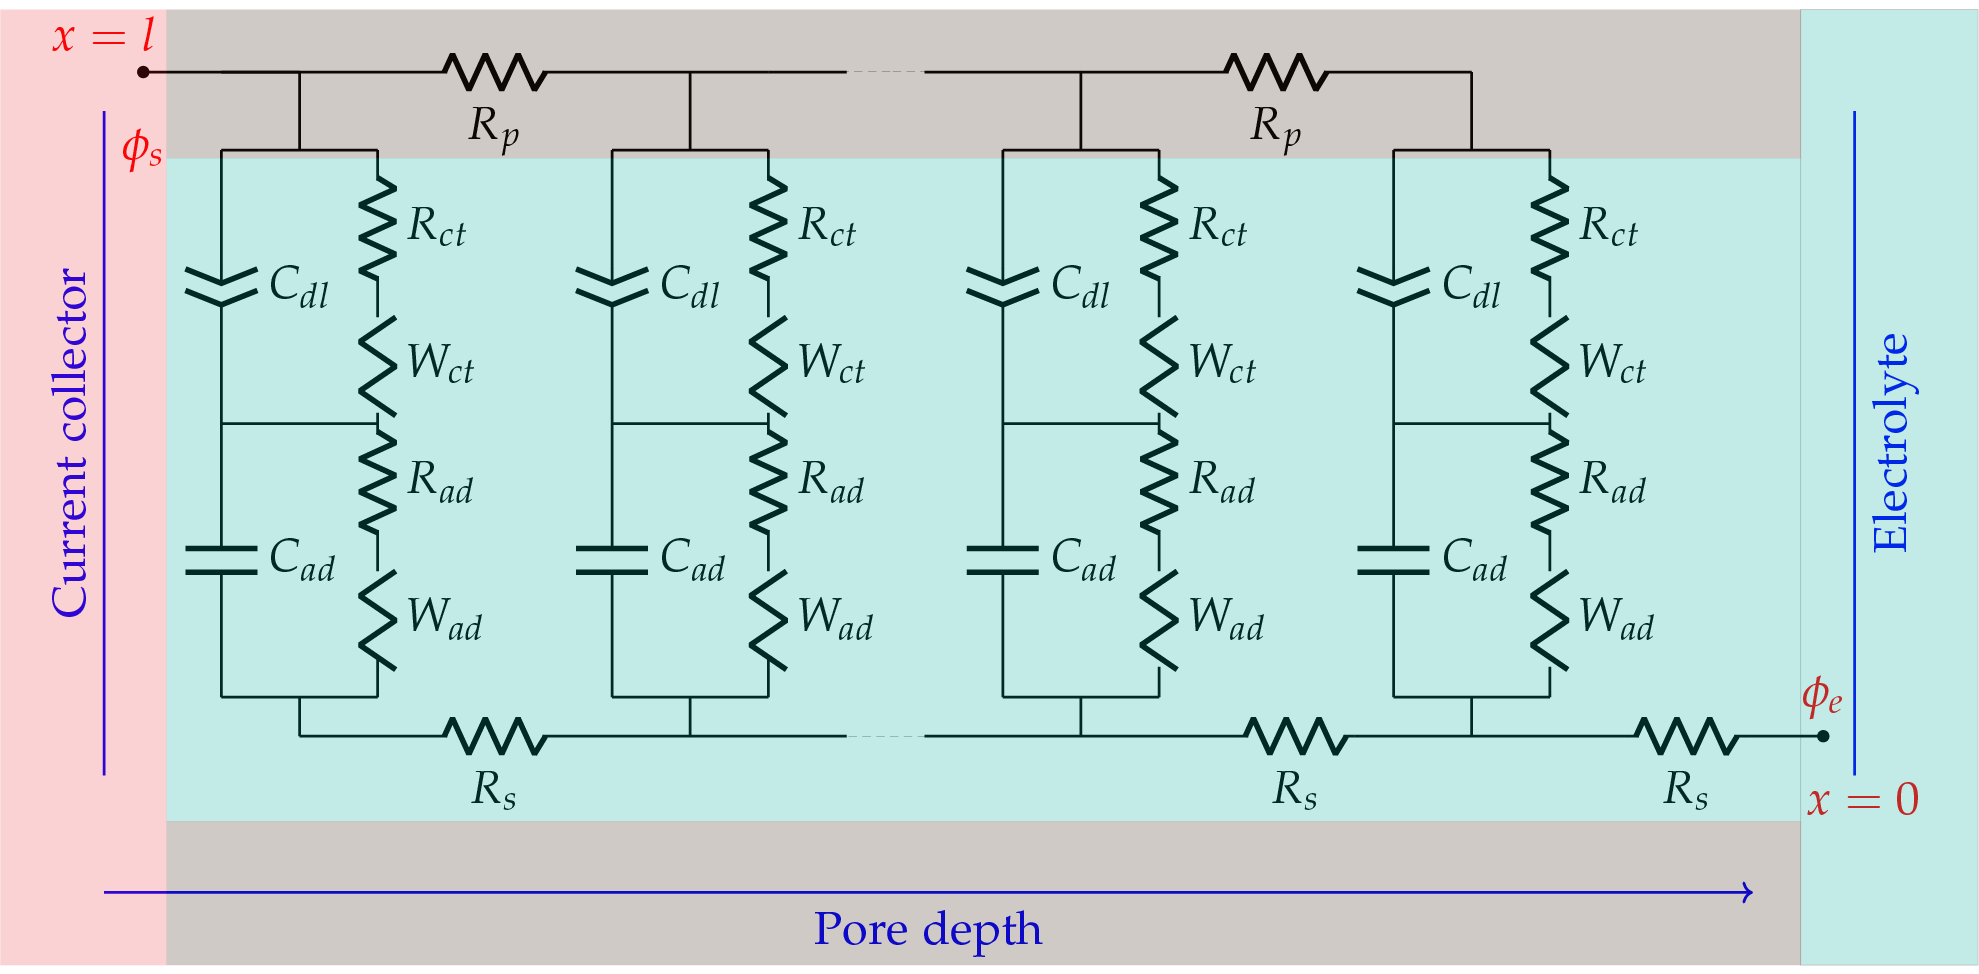
\includegraphics[width=\textwidth]{figures/LTP/ltp_circuit_new.png}
    \label{fig:LTP circuit}
    \caption{Equivalent circuit of the physical model used to fit DEIS spectra.}
\end{figure}

The interface processes are described by the following simplified unit (Figure \ref{fig:LTP circuit simplified}) in the transmission line where the Warburg element rapresenting the charge trasnfer has been substituteby a capacitor. This semplification produces better fit with lower ammount of paramters.

\begin{figure}[h!]
    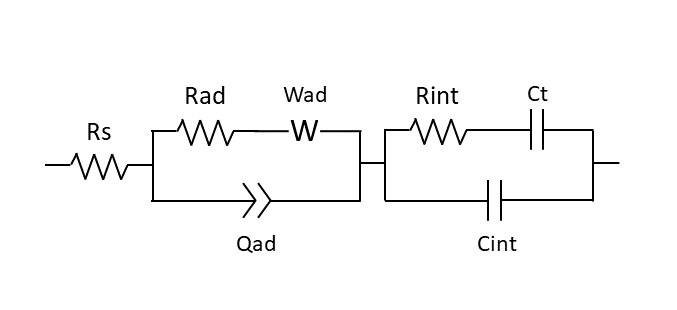
\includegraphics[width=0.8\textwidth]{figures/LTP/EC_collins_simplified.jpg}
    \caption{Equivalent circuit of the physical model developed for the intercalation processes of MnO2 in \cite{erinmwingbovoDynamicImpedanceSpectroscopy2020}}
    \label{fig:LTP circuit simplified}
\end{figure}


\subsubsection{Simplified model for time-varying impedance}

For the dynamic impedance measurements presented in this work (Chapters 10-11), a simplified version of this model was employed. At frequencies above the diffusion regime but below where inductive effects dominate, the impedance can be approximated by:

\[
Z(\omega) = R_s + \frac{R_{pore}}{\sqrt{1 + j\omega\tau_{pore}}} + \frac{R_{ct}}{1 + j\omega R_{ct}(C_{dl} + C_\mu)}
\]

where:
\begin{itemize}
\item $R_s$ is the solution resistance (ohmic drop)
\item $R_{pore}$ captures the distributed pore resistance
\item $\tau_{pore} = R_e C_{dl}$ is the characteristic pore time constant
\item The third term represents the charge transfer process coupled with both double-layer and chemical capacitance
\end{itemize}

This form yields a characteristic impedance spectrum with:
\begin{enumerate}
\item A high-frequency intercept corresponding to $R_s$
\item A depressed semicircle in the mid-frequency range from the porous electrode behavior
\item A second semicircle or Warburg-like tail at low frequencies from charge transfer and diffusion
\end{enumerate}

\subsubsection{Application to lithium titanium phosphate}

For the LiTi$_2$(PO$_4$)$_3$ electrodes studied in Chapter 10, this model was fitted to dynamic impedance data acquired during both galvanostatic and voltammetric perturbations in aqueous sodium-ion electrolyte. The key findings were:

\begin{itemize}
\item $R_{ct}$ varies significantly with state of charge, reflecting the potential-dependent kinetics of Na$^+$ insertion
\item An asymmetry was observed between charge and discharge, attributed to differences in solvation/desolvation activation energies
\item The porous electrode contribution ($R_{pore}$) remained relatively constant, confirming good ionic connectivity throughout cycling
\item Chemical capacitance $C_\mu$ peaks near 50\% state of charge, consistent with the voltage plateau region where the thermodynamic factor $\partial \mu / \partial c$ is maximized
\end{itemize}

This physical interpretation was only possible due to the use of a three-electrode configuration with a properly positioned reference electrode, enabling separation of the working electrode impedance from the counter electrode contribution.

\subsubsection{Model for electrical double-layer capacitors}

For the symmetric activated carbon electrodes (Chapter 11), a similar porous electrode framework applies, but without the Faradaic charge transfer term. The impedance simplifies to:

\[
Z(\omega) = R_s + \frac{R_{pore}}{\sqrt{1 + j\omega\tau_{pore}}} + \frac{1}{j\omega C_{dl,eff}}
\]

where $C_{dl,eff}$ is the effective double-layer capacitance of the porous structure. The model accounts for:

\begin{itemize}
\item Ion adsorption/desorption at the carbon surface (non-Faradaic process)
\item Distributed ionic resistance within the nanoporous carbon network
\item Frequency dispersion due to pore size distribution (often modeled with constant phase elements)
\end{itemize}

Despite using chemically identical electrodes, the positive and negative electrodes exhibited different impedance magnitudes and time constants during cycling, attributed to:
\begin{enumerate}
\item Different electrochemical histories (voltage excursions)
\item Adsorption of electrochemically inactive species (e.g., oxygen reduction products at positive electrode)
\item Asymmetric ion accessibility at different potentials
\end{enumerate}

The time-varying impedance revealed that these effects evolve continuously during charge/discharge, information that would be invisible in traditional equilibrium measurements.

% \section{Simultaneous fitting}

% The approach of fitting for dynamic impedance is similar to what is commonly done for static impedance, but there is the challenge that for a non-stationary experiment the dynamic of the system can change with the activation or deactivation of chemical processes with time, voltage or temperature. For example, a battery would change its state of charge during a galvanostatic technique and the system response might change at different potential, and with its cycling history.  The common approach, sometimes called batch fitting, would be of fitting one spectra of the time using the optimized parameters of the previous spectra for the following. The problem is that some parameter of the model would be close to zero in some part of the dataset and potentially very big in others. Solving optimization problems with small and redundant parameters might lead to local solutions. Furthermore, when more than one parameter is of this type, the solver might converge to different minimum for each spectra even when the optimized parameters of the prevoious spectra are used as starting points. This issue can be addressed minimizing the entire dataset at ones and introducing a regularization term in the objective function as firstly introduced by Battistel et al. The objective function become: \\

% equation?\\

% Intuitively, one can consider a term that minimizes the distance between data points and model while another term keeps the parameters slowly evolving across the dataset. The penalty term avoids sudden variation of parameters that arises in those areas of the dataset where there is unavoidable overparametrization.
% Recently Cuckwu extended the concept of  penalized objective function implementing modern methods to solve high dimensional optimization problem as used in the field of Machine Learning. An improvement in computation time for big dataset has been obtained combining the efficient methods for calculating derivatives called "automatic gradient" or automatic differentiation and the solver ADAM. Both can be find in the open source package JAX that uses the Python pre-compiling from the jit library to perform the calculation in multiple threads, processors or even distributed computing (including GPUs). JAX is supported for optimization-specific problems in the open source package Optax. Cuckwu implementation is open source but compatible up to Python 3.9 and only with JAXopt, the previous project from which Optax derived (not in development anymore). Dr. Nicoló Pianta updated Chucwu's code base to modern version and added a convenient object rapresentation for the model function, similar to the well-enstablished python library for non linear fitting nlfit. For each experiment of the Applications part I will specify which library was used to analyze the impedance.\\

\subsection{Fitting error}
We estimate the standard deviation from the Jacobian of the objective function. The error allows to verify in most of the cases the accuracy of the model and which parameters are not significant in the estimation.

\section{Determination of the system degrees of freedom}

When fitting physical models, the user decides \emph{a priori} the degreese of freedom of the system though the number and types of approximation and the equation that chose to keep. The process of model regression gives to the scientist a confirmation that the model can represent the nature of the system under the operating condition or not. On negative result one keeps modifying the model until satisfied. On the other hand, when working with black-box model the scientist makes the opposite: identifies the degreese of freadom of the system and then look for a proper gray-box or white-box model of the same structure to undenstand the physics of the system.  This data driven apporach relies on the fact that the frequency reponse function is a numerical realization of the real transfer function of the system inside the frequency band of the experiment. From dynamic system theory it is known that the number of parameters of the transfer function is equal to the number of variables in the state space model, directly connected to the differential equations that define the system. For batteries, that works as two-electrode devices, the response of the single electrode is superimposed making even harder to define a general physical model. Usually the model are largely over-parametrized. Knowing the correct transfer function, leads scientists to chose proper approximation when developing physical model or can be is as it for prediction or classification of the system in control engeneering. It immediatly come to mind the possibililty of using it for smart control of the battery in battery managment systems. 

\section{Determining transfer function structure}
The identification of the transfer function structure is the process of finding the order of the nominator and denominator of the polynomial rational function through statistical approach. In this work I ... 